\chapter{Query Recency Sensitivity Model}
\label{ch:query}

\definecolor{eclipseStrings}{RGB}{42,0.0,255}
\definecolor{eclipseKeywords}{RGB}{127,0,85}
\colorlet{numb}{magenta!60!black}
\colorlet{punct}{red!60!black}
\definecolor{delim}{RGB}{20,105,176}

\lstset{
  basicstyle=\ttfamily,
  columns=fullflexible,
  showstringspaces=false,
  commentstyle=\color{gray}\upshape,
  breaklines=true
}
\lstdefinelanguage{bash}
{
%     morestring=[b]",
%     morestring=[d]'
  commentstyle=\color{eclipseStrings}, % style of comment
  stringstyle=\color{eclipseKeywords}, % style of strings
  numbers=left,
  frame=lines,
  %backgroundcolor=\color{gray}, %only if you like
  string=[s]{"}{"},
  comment=[l]{:\ "},
  morecomment=[l]{:"},
  moredelim=**[is][\color{blue}]{?}{?},
  moredelim=**[is][\color{orange}]{!}{!},
  moredelim=**[is][\color{red}]{^}{^}
}

A web search query is a query that a user enters into a web search engine to satisfy their information needs. As described by \citet{broder2002taxonomy}, queries have empirically been divided into three different groups:
\begin{itemize}
	\item Informational queries: queries that cover a broad topic for which there may be thousands of relevant results (e.g., \textit{barcelona}).
	\item Navigational queries: queries that seek a single website or web page of a single entity (e.g., \textit{youtube}, \textit{facebook}).
	\item Transactional queries: queries that reflect the intent of the user to perform a particular action, such as downloading a screen saver.
\end{itemize}

Another possible division of queries can be according to their temporal profiles, as defined by \citet{jones2007temporal}. They propose three temporal classes of queries:
\begin{itemize}
	\item Atemporal queries: queries that take place at any time.
    \item Temporally unambiguous queries: queries that take place at a specific period in time.
    \item Temporally ambiguous: queries that take place during one of several possible episodes.
\end{itemize}

\begin{figure}
\centering
\begin{subfigure}{.5\textwidth}
  \centering
  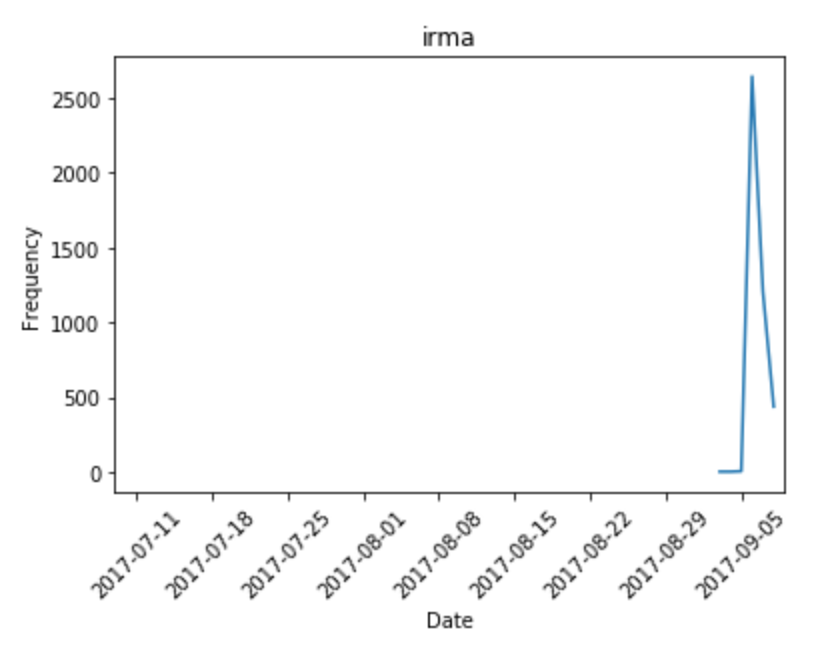
\includegraphics[width=.8\linewidth]{img/query1.png}
  \caption{A temporally unambiguous query.}
  \label{fig:query1}
\end{subfigure}%
\begin{subfigure}{.5\textwidth}
  \centering
  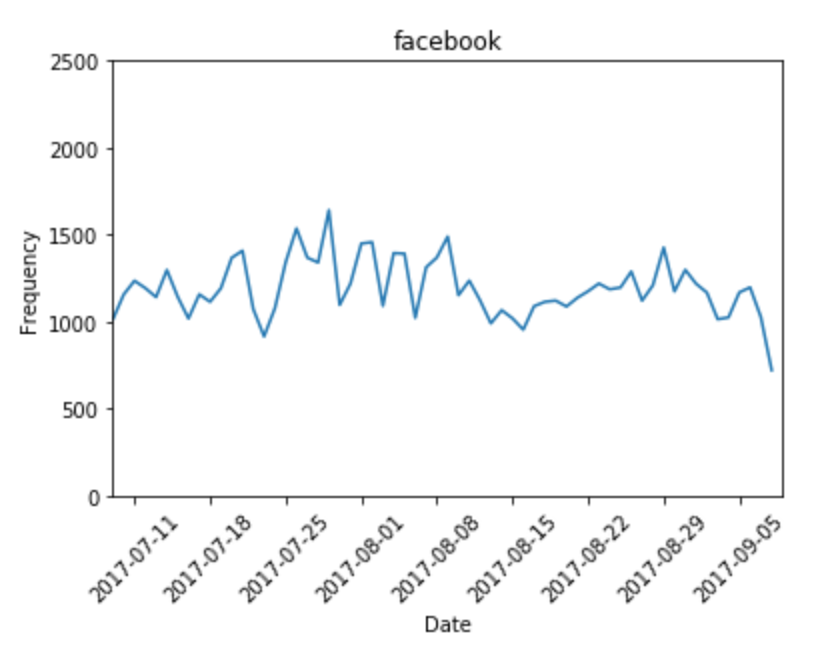
\includegraphics[width=.8\linewidth]{img/query2.png}
  \caption{An atemporal query.}
  \label{fig:query2}
\end{subfigure}
\caption{Examples of queries with different temporal profiles.}
\label{fig:query-temporal}
\end{figure}

Figure \ref{fig:query-temporal} shows an example of queries with different temporal profiles. The query \textit{irma} is temporally unambiguous, as it refers to the hurricane Irma, whereas the query \textit{facebook} is atemporal.

User experience is improved by integrating recency of retrieved results for most types of queries. Therefore, instead of focusing on a specific query type, we choose to introduce the recency vertical for queries in general.

As described by \cite{styskin2011recency}, not all queries require the same percentage of recent results, and not all queries seek the same granularity of result recency (e.g., hours, days, years). We call this property \textit{query recency sensitivity}. We argue that the inference of query's recency sensitivity has an impact on the ranking of retrieved results.

In a conventional information retrieval setting, a query instance is defined only as the query string. However, as we are introducing a recency component, we have to capture the temporal aspect of the query as well. For example, for the query \textit{stephen hawking}, the user might expect little to no change in results when submitting the same query in different points in time. Nonetheless, if searching for \textit{stephen hawking} on March 14, 2018, we would expect to see more breaking-news results than usually, since that was the day he died. Thus, in a query recency sensitivity setting, we define a query instance as:
\[ queryInstance = (queryText, submissionTime) \]

\noindent In other words, the same query can be submitted at different times, and yield a different ranking of results. \citet{styskin2011recency} also defined different levels of recency sensitivity. They define four labels of recency sensitivity and ask human judges to annotate real user queries. The labels are probabilities from $[0,1]$, and are defined as the following:
\begin{enumerate}
	\item \texttt{0.95}: the query is strictly about a recent event, e.g., \textit{stephen hawking death} on the day of the event;
    \item \texttt{0.75}: the query's primary interest is related to a recent event, but the user also wants just topically relevant results, e.g., \textit{oscar} on the day of the ceremony;
    \item \texttt{0.25}: the query’s primary interest is not likely to be focused on a particular event, but it makes sense to present some recent content, e.g., \textit{britney spears};
    \item \texttt{0}: otherwise, the query is assigned zero probability to be recency sensitive.
\end{enumerate}

\noindent We use these observations in constructing our ground truth dataset.

\section{Ground Truth Creation}
Instead of manually annotating queries, we choose to automatically infer recency sensitivity for queries. For this, we use a previously compiled ground truth dataset used for web ranking evaluation.\footnote{The details of this dataset cannot be disclosed, as it was constructed within a commercial project.} The dataset consists of $142807$ queries submitted to a third party search engine in the period of July 2017 -- September 2017.

Unfortunately, when this dataset was compiled, the query submission date was not recorded, as it was deemed unnecessary for relevance-based ranking evaluation. However, we were able to reconstruct it based on the order in which the queries were submitted, the rate they were submitted at, and the start and end date of the scraping. Since we are only able to reconstruct the submission date, not the exact time, we set the time as 23:59 of that day.

The queries were submitted to a third party search engine, and the first 50 results per query were scraped. An example of a partial result set for the query \textit{kardashian} is shown in Listing~\ref{serp}.

\begin{lstlisting}[language=json,firstnumber=1,caption=Example of retrieved results for a query., label=serp]]
{
  query_text: "kardashian",
  query_submission_date: "2017-08-27 23:59:00",
  results: {
    list: [
      {
        rank: "0",
        uri: "https://www.instagram.com/kimkardashian/?hl=en",
        title: "Kim Kardashian West (@kimkardashian): Instagram photos and videos",
        snippet: "103m Followers, 111 Following, 3933 Posts - See Instagram photos and videos from Kim Kardashian West (@kimkardashian)"
      },
      {
        rank: "1",
        uri: "https://en.wikipedia.org/wiki/Kim_Kardashian",
        title: "Kim Kardashian - Wikipedia",
        snippet: "Kimberly Kardashian West is an American reality television personality, socialite, actress, businesswoman and model. Kardashian first gained media attention..."
      },
      {
        rank: "2",
        uri: "http://people.com/babies/kanye-west-kim-kardashian-expecting-third-child-surrogate-pregnant/",
        title: "Kanye and Kim Kardashian West Expecting Third Child - People",
        snippet: "19 hours ago - Kim Kardashian and Kanye West Expecting Baby No. 3 via Surrogate! ..."
      },
      {
        rank: "3",
        uri: "http://people.com/babies/kim-kardashian-first-red-carpet-appearance-baby-number-3/",
        title: "Kim Kardashian Makes First Red Carpet Appearance Following News ...",
        snippet: "10 hours ago - Kim Kardashian West made her first red carpet appearance at New York Fashion Week on Wednesday following the news that she is expecting..."
      }
      (...)
    ]
  }
}
\end{lstlisting}

The snippet field shows the beginning of the document, and sometimes it includes information on when the document was published. This timestamp is relative to the query submission date, and can be in the form of \texttt{1-23 hours ago}, \texttt{2-7 days ago}, or a specific date, i.e., \texttt{May 27, 2018}. We take advantage of this temporal information when automatically determining which queries are more recency sensitive than others.

Our idea is to sort the queries in descending order based on a custom recency sensitivity function, then apply labels based on the distribution of the classes shown in Figure \ref{fig:query_dis}, and defined by \citet{styskin2011recency}. To score a query, we first take all the results with snippets that contain \texttt{1-23 hours ago}. We convert the relative timestamp to an absolute one by subtracting its value from the query submission time and express it as Unix time. We define the query score as the sum of the timestamps from the described snippets. Lastly, we sort the queries according to this score in descending order, and assign the label \texttt{0.95} to the first 0.73\% of queries, \texttt{0.75} to the next 1.11\%, \texttt{0.25} to the next 4.9\%, and \texttt{0.0} to the rest. Next, we downsample our query set from the initial $142807$ queries to $4000$ by maintaining the distribution of classes. Finally, we use this as ground truth for the query recency sensitivity model.

\begin{figure}
  \centering
  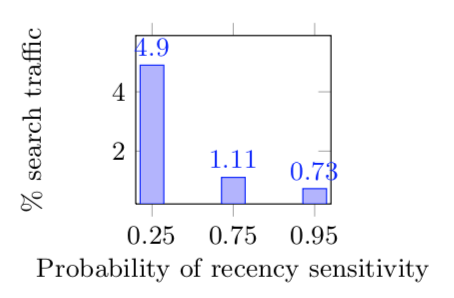
\includegraphics[width=0.4\textwidth]{img/query_distribution.png}
  \caption{Distribution of query recency sensitivity classes defined by \citet{styskin2011recency}.}
  \label{fig:query_dis}
\end{figure}

\section{Feature Extraction}

We use 34 features in our model. We extract features from three different sources:
\begin{itemize}
	\item Our query log. Features such as the number of times the query was submitted over different time periods, and the ratio of the number of submissions of the query in the last day and in the last week. Additionally, the probabilities of the query being generated by language models based on the query log over different time periods.
    \item The query itself. These are features such as the number of tokens, and several boolean features.
    \item Twitter. We mine recent tweets with respect to the query submission time, and generate language models based on tweets in the last day, week, and two weeks.
\end{itemize}

A comprehensive list of features can be seen in Table~\ref{tb:features-query}. Here, the first six features are extracted from the query log, the next four features from the query itself, and the rest of the features are probabilities of the query being generated by different language models. Language models built on tweets and using bigrams are denoted as \texttt{LM\_Tweet\_2}, and the ones using trigrams are \texttt{LM\_Tweet\_3}. The same applies for language models built on the query log, denoted as \texttt{LM\_QL}.

\begin{table}[]
\centering
\caption{List of features.}
\label{tb:features-query}
\begin{tabular}{@{}cl@{}}
\toprule
Feature index & Feature name \\ \midrule
1 & QuerySubmissions\_LastDay \\
2 & QuerySubmissions\_LastWeek \\
3 & QuerySubmissions\_LastMonth \\
4 & QuerySubmissions\_Day/Week \\
5 & QuerySubmissions\_Day/Month \\
6 & QuerySubmissions\_Week/Month \\
7 & Contains\_News \\
8 & Contains\_Now \\
9 & Contains\_Numeral \\
10 & NumberTokens \\
11 & LM\_Tweet\_2\_Day \\
12 & LM\_Tweet\_2\_Week \\
13 & LM\_Tweet\_2\_TwoWeeks \\
14 & LM\_Tweet\_2\_Day/Week \\
15 & LM\_Tweet\_2\_Day/TwoWeeks \\
16 & LM\_Tweet\_2\_Week/TwoWeeks \\
17 & LM\_Tweet\_3\_Day \\
18 & LM\_Tweet\_3\_Week \\
19 & LM\_Tweet\_3\_TwoWeeks \\
20 & LM\_Tweet\_3\_Day/Week \\
21 & LM\_Tweet\_3\_Day/TwoWeeks \\
22 & LM\_Tweet\_3\_Week/TwoWeeks \\
23 & LM\_QL\_2\_Day \\
24 & LM\_QL\_2\_Week \\
25 & LM\_QL\_2\_Month \\
26 & LM\_QL\_2\_Day/Week \\
27 & LM\_QL\_2\_Day/Month \\
28 & LM\_QL\_2\_Week/Month \\
29 & LM\_QL\_3\_Day \\
30 & LM\_QL\_3\_Week \\
31 & LM\_QL\_3\_Month \\
32 & LM\_QL\_3\_Day/Week \\
33 & LM\_QL\_3\_Day/Month \\
34 & LM\_QL\_3\_Week/Month \\ \bottomrule
\end{tabular}
\end{table}

\subsection{Language Model Features}

Language models are models that assign probabilities to sequences of words, or in our case, queries. We use language models to determine the probability of a query being generated by a set of tweets or queries in our query log over different time periods.

Formally, an $n$-gram language model makes the assumption that the probability of a word only depends on the previous $n$ words. Therefore, the probability $P(w_{1},\ldots ,w_{m})$ of observing the sentence $w_{1},\ldots ,w_{m}$ is approximated as:
\[ P(w_{1},\ldots ,w_{m})=\prod _{{i=1}}^{m}P(w_{i}\mid w_{1},\ldots ,w_{{i-1}})\approx \prod _{{i=1}}^{m}P(w_{i}\mid w_{{i-(n-1)}},\ldots ,w_{{i-1}}) \]

\noindent The conditional probability can be calculated from $n$-gram model frequency counts:
\[ P(w_{i}\mid w_{{i-(n-1)}},\ldots ,w_{{i-1}})={\frac  {{\mathrm  {count}}(w_{{i-(n-1)}},\ldots ,w_{{i-1}},w_{i})}{{\mathrm  {count}}(w_{{i-(n-1)}},\ldots ,w_{{i-1}})}} \]

A common problem when using frequency counts directly is the sparsity of the data. In other words, many words will yield zero and the overall probability will be zero. To prevent this, a technique called \textit{smoothing} is used to assign some probability to unseen words. Various techniques exist, the simplest one being \textit{add-one smoothing}, or assigning a count of 1 to unseen words. The most commonly used technique is the interpolated Kneser-Ney algorithm \citep{kneser1995improved}.

We use the KenLM Language Model Toolkit\footnote{\url{https://kheafield.com/code/kenlm/}.} to construct our language models. The toolkit uses linear probing for storing the frequency counts and the Kneser-Ney algorithm for smoothing. The toolkit is decribed in detail in \citep{Heafield-kenlm} and \citep{Heafield-estimate}. The usage is straightforward and consists of two steps: estimating (building) the language models, and querying them (producing probabilities for queries).

An example for a bigram language model is shown in Listing \ref{kenlm}. First, we estimate a language model by providing a corpus (in our case either tweets or queries in our query log), and the order of the model (in this case, two for bigrams). Next, we convert the produced ARPA file to a binary format to reduce loading time. Finally, we query the model by providing the queries as input, and get probabilities of the queries being generated by that language model as the output.

\begin{lstlisting}[language=bash,firstnumber=1,caption=Estimating a bigram language model and producing predictions for queries., label=kenlm]]
?kenlm/bin/lmplz? !-o! 2 < INPUT_CORPUS > model.2.arpa
?kenlm/bin/build_binary? model.2.arpa model.2.binary
?kenlm/query? !-v! sentence model.2.arpa < INPUT_QUERIES > OUTPUT_PROBABILITIES
\end{lstlisting}

\subsubsection{Query log corpus}
We estimate language models based on our query log by first extracting the corresponding corpus. For a date $d$, we create language models based on the queries in our query log from the previous day, week, and month. As explained earlier, our ground truth consists of queries submitted in the period of July 2017 -- September 2017. For each date $d$ from this time period, we model three different time slots $t$, and two different types of language models, bigrams and trigrams, which amounts to six language models per date $d$.

Inspired by \citet{dong2010towards}, our idea is to compare the probabilities for the input query to be generated by language models $LM_{Q,t}$, where $t \in \{\text{prev\_day}, \text{prev\_week}, \\ \text{prev\_month}\}$. If there is a spike in interest for a given query, resulting in more traffic and, consequently, higher need for recent results, we expect the probability of $LM_{Q,{\rm prev\_day}}$ to be higher than $LM_{Q, {\rm prev\_week}}$ and especially $LM_{Q, {\rm prev\_month}}$. Features with indices 23--34 in Table \ref{tb:features-query} model the probabilities of different $LM_{Q,t}$, as well as their ratios.

\subsubsection{Twitter corpus}
Similar to the query log corpus, our idea is to extract a corpus of tweets from different time slots, construct language models, and model the probabilities for the input query to be generated by these language models. In this case, we build language models $LM_{T,t}$, where $t \in \{\text{prev\_day}, \text{prev\_week}, \text{prev\_two\_weeks}\}$. Features with indices 11--22 in Table \ref{tb:features-query} model the probabilities of different $LM_{T,t}$, as well as their ratios.

For the queries in our ground truth, collecting the tweets is simple since we are able to do it in an offline manner. More specifically, we download a precompiled archive of tweets produced by The Internet Archive,\footnote{\url{https://archive.org/about/}.} a nonprofit digital library. They provide monthly archives of tweets, sampled from the general Twitter stream, as a simple collection of JSON objects.

In an online setting, where we cannot download a precompiled archive, we use a Python library called \texttt{twarc}\footnote{\url{https://github.com/docnow/twarc}.} to grab fresh tweets. The library queries the Twitter API, handles Twitter API's rate limits, and stores the retrieved tweets as JSON objects. Before querying the API, we register our developer application with Twitter to use the Standard search API,\footnote{\url{https://developer.twitter.com/en/docs/tweets/search/api-reference/get-search-tweets}.} which means we are able to retrieve only the past seven days of tweets. 

We contributed to this library by adding the parameter \texttt{until}, which is a date specifying the cut-off date for tweet creation date. This option was needed because \texttt{twarc} downloads tweets for a specific date until exhaustion, which takes too long, so we decide to run the tweet retrieval separately for each day in the past week. Moreover, the library does not support stopping after retrieving a certain number of tweets, so we used the \texttt{timeout.sh} script written by Anthony Thyssen\footnote{\url{http://www.ict.griffith.edu.au/anthony/software/#timeout}.} to terminate the process after a certain time elapsed. An example of collecting tweets from a specific date is shown in Listing \ref{twarc}.

\begin{lstlisting}[language=bash,firstnumber=1,caption=Downloading a collection of tweets for a specific date using \texttt{twarc}., label=twarc]]
?twarc configure?
?./timeout.sh? 14400 ?twarc search? 'a OR b OR c OR d OR e OR f OR g OR h OR i OR j OR k OR l OR m OR n OR o OR p OR q OR r OR s OR t OR u OR v OR w OR x OR y OR z' !--lang! en !--until! 2018-06-13 !--log! 2018-06-12.log > tweets-2018-06-12.json
\end{lstlisting}

Since the library does not support searching all tweets without a search query, we search for any tweet consisting of any of the characters from the English alphabet. Next, the parameter for timing out is given in seconds, and $14400$ seconds is equivalent to $4$ hours, which is the time it takes to download $\sim300K$ tweets created in a given day. The parameters for \texttt{twarc} are \texttt{log}, the path to the log file, and \texttt{lang} specifying the language of tweets to retrieve. In this work, we only focus on English.

\subsection{Other Features}
Other features are represented with indices 1--10 in Table \ref{tb:features-query}. The first six are extracted from the query log, and represent the number of query submissions in the past day, week, and month, as well as their ratios. Intuitively, we can imagine that queries related to new events would have a spike in popularity. Moreover, boolean features 7--9 check if the query contains the word \textit{news}, \textit{now}, or a numeral. The last feature in this group is the number of tokens in the query.

\section{Model Training}
We use XGBoost (eXtreme Gradient Boosting), introduced by \citet{chen2016xgboost}, an open-source parallel gradient boosting library to train and evaluate the model. Even though our ground truth labels are four classes with values ranging from \texttt{0} to \texttt{0.95}, we formulate this as a regression problem and train a model to predict a query recency sensitivity score between \texttt{0} and \texttt{1}. To this end, we build Gradient Boosted Regression Trees (GBRT).

We have a total of 34 features, where each feature value is numerical. The training instances are of the \texttt{LibSVM data format}:\footnote{\url{https://www.csie.ntu.edu.tw/~cjlin/libsvm/}.}
\[ \texttt{<label> <index\_1>:<value\_1> ... <index\_N>:<value\_N>} \]

Here, \texttt{<label>} is the target value, a number between 0 and 1, and the rest of the fields model the feature index and value, respectively.

To determine which features are more useful than others, we plot the feature importance scores, as seen in Figure \ref{fig:fscores-queries}. Cross-referencing with Table \ref{tb:features-query}, we can see that the feature with index $16$, \texttt{LM\_Tweet\_2\_Week/Month} is the most useful one. This confirms our intuition that the higher the ratio of probabilities of the more recent language model and the older the language model is, the more recency sensitive the query is. The other most important features are \texttt{LM\_Tweet\_2\_Day}, \texttt{LM\_Tweet\_2\_Week}, \texttt{LM\_QL\_2\_Day/Week}, \texttt{LM\_Tweet\_3\_TwoWeeks}, \texttt{LM\_Tweet\_3\_Week} and \texttt{LM\_Tweet\_3\_Week/TwoWeeks}. This indicates that language models are strong features, both those consisting of bigrams and trigrams.

On the other end, the worst performing features are boolean features \texttt{Contains\_Now} and \texttt{Contains\_Numeral}. It was expected that the boolean features would not have a great impact, as they are cheap to compute and very simple. Following these, the other worst performing features come from the query log, \texttt{QuerySubmissions\_Day/Week} and \texttt{ QuerySubmissions\_Day/Month}. This may be because our query log is too sparse to provide meaningful features.

\begin{figure}
  \centering
  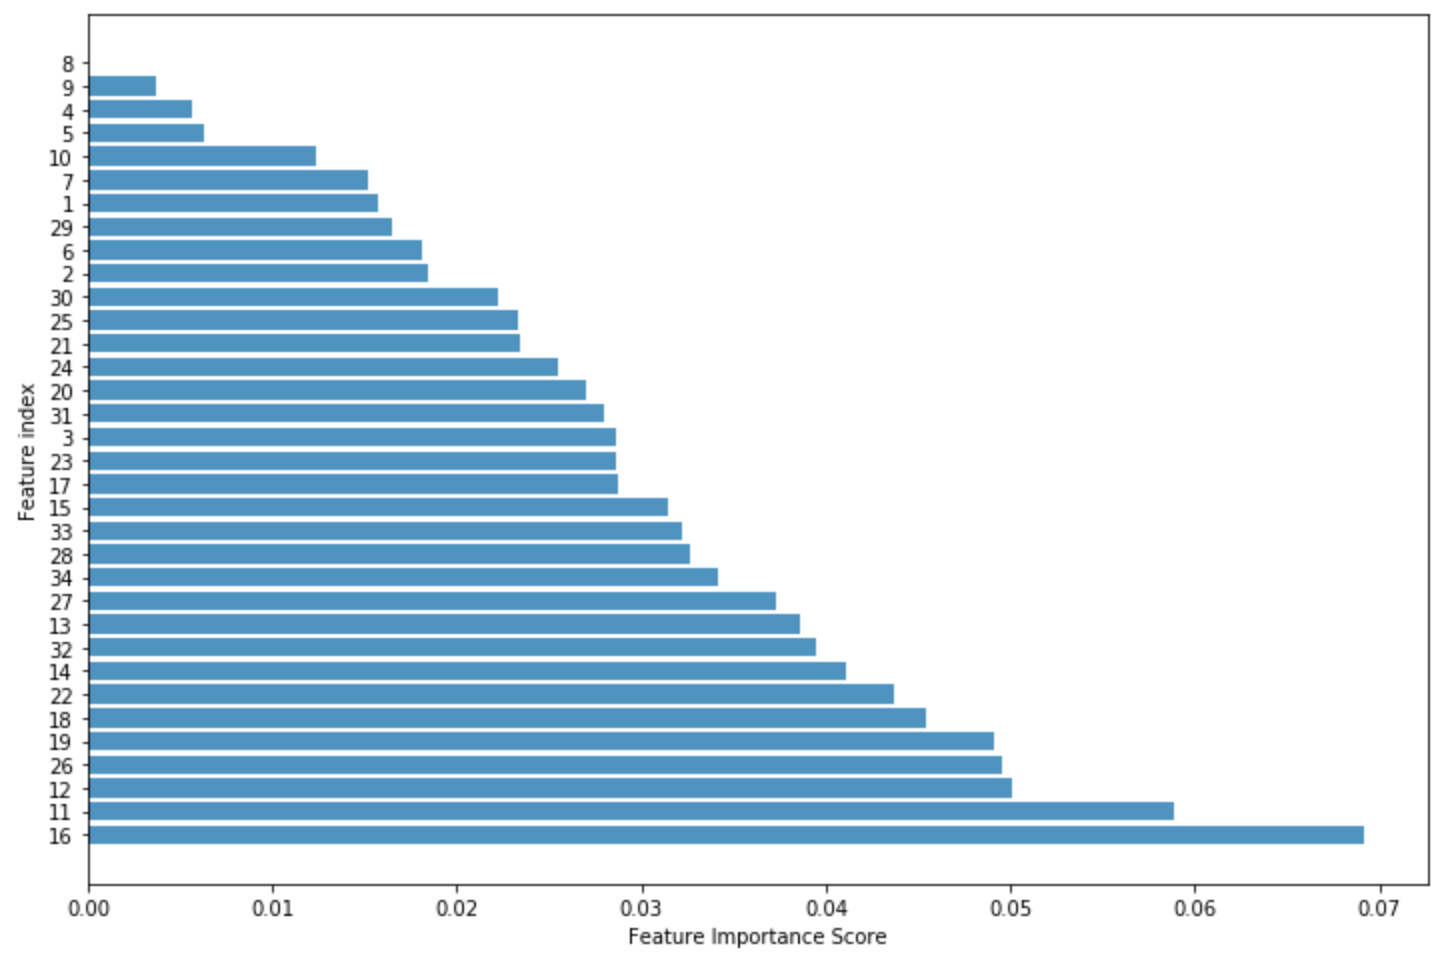
\includegraphics[width=\linewidth]{img/query_f_importance.png}
  \caption{Feature importance scores for the query recency sensitivity model.}
  \label{fig:fscores-queries}
\end{figure}
% plotted in queries.ipynb

We plot the first tree created in the model to gain insight into the decision process. The tree is shown in Figure \ref{fig:query_tree0}. We can see that the first decision is based on feature 10, but as the features are 0-indexed in the implementation, this is actually feature with index 11 from Table \ref{tb:features-query}, \texttt{LM\_Tweet\_2\_Day}. The next level is based on features with indices 1 and 2, \texttt{QuerySubmissions\_LastDay} and \texttt{QuerySubmissions\_LastWeek}. Arriving to the first leaf of the tree, the model concludes that if the probability of the language model based on bigrams from tweets from the past day is lower than a certain threshold, and the query was submitted less than 8 times in the past week, the resulting contribution to the overall score is 0.002, a very small value.

\begin{figure}
  \centering
  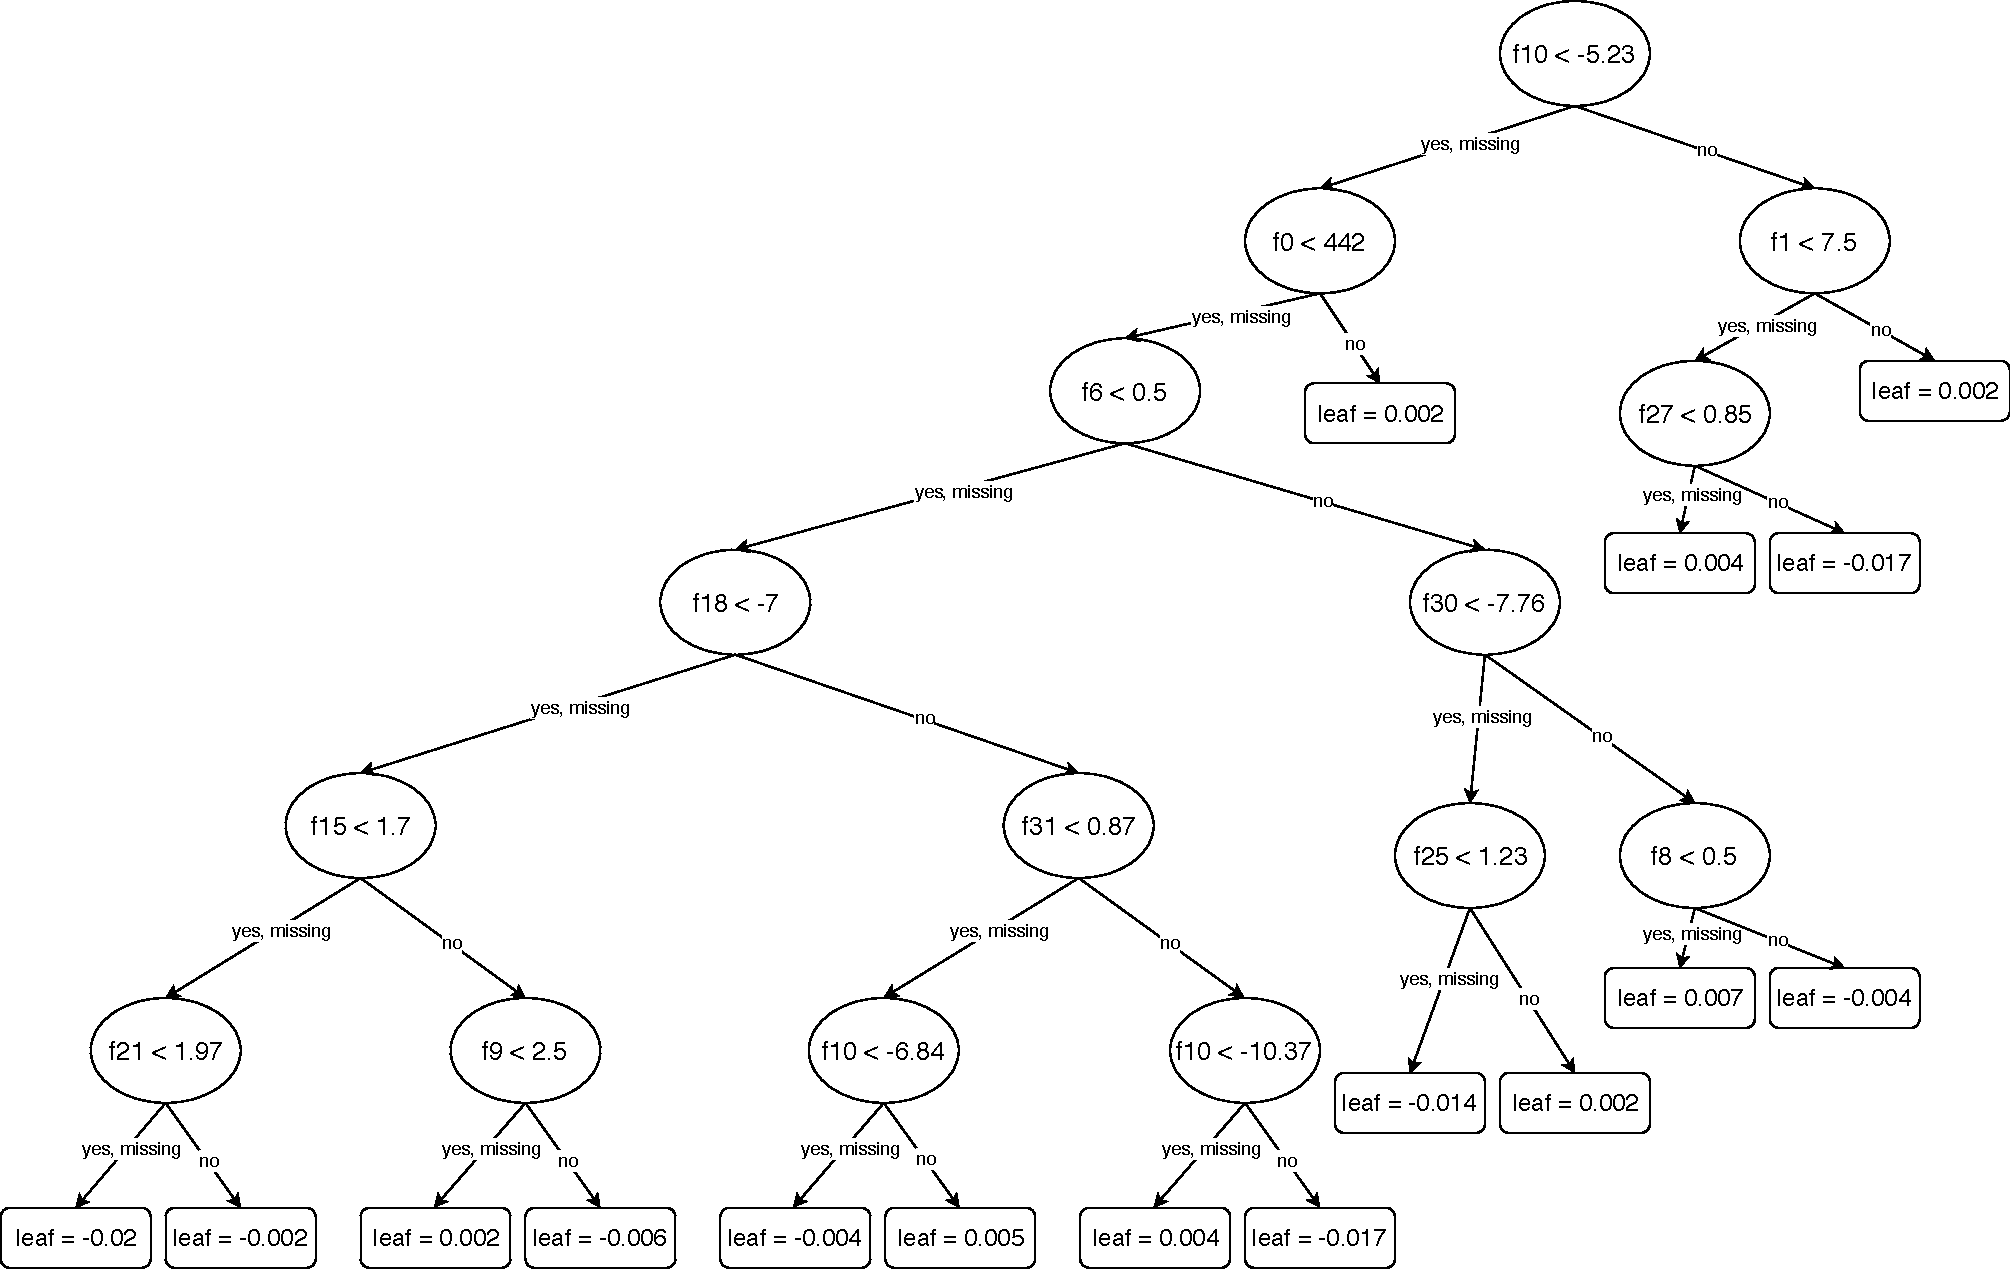
\includegraphics[width=\linewidth]{img/tree.pdf}
  \caption{First tree of the query recency sensitivity model.}
  \label{fig:query_tree0}
\end{figure}

\section{Evaluation}
For training the model, we split the input set into train and validation sets in the 70:30 ratio. We then proceed to grid search the hyper-parameters of the model using a 5-fold cross-validation. Listing~\ref{param-query} shows which hyper-parameters are tuned.

\begin{lstlisting}[language=json,caption=Hyper-parameter tuning for the query recency sensitivity model.,label=param-query]
'max_depth': [4, 6, 8, 10],	(best = 6)
'min_child_weight': [0, 1, 2],	(best = 0)
'gamma': [0.0, 0.1, 0.2, 0.3],	(best = 0.0)
'subsample': [0.6, 0.8, 1.0],	(best = 0.6)
'colsample_bytree': [0.6, 0.8, 1.0],	(best = 0.6)
'learning_rate': [0.01, 0.03, 0.1, 0.2, 0.3],	(best = 0.01)
'n_estimators': [100, 500, 1000, 5000]	(best = 500)
\end{lstlisting}

%  Best hyperparameters:
% {'colsample_bytree': 0.6, 'learning_rate': 0.01, 'min_child_weight': 0, 'n_estimators': 500, 'subsample': 0.6, 'max_depth': 6, 'gamma': 0.0}
% RMSE (train) 0.084499281335
% RMSE (test): 0.1077
% 1706.14706233

The hyper-parameters are explained in detail earlier in the thesis, in Section~\ref{sec:docparams}. We also set the model to stop learning if there are not any improvements after 50 rounds.

The training of the model took 28 hours on a machine with CentOS 7.5.1804, 16 GB of RAM, and 8 Intel(R) Xeon(R) CPU E5-2660 v3 @ 2.60GHz CPUs. The model was trained by minimizing the root mean squared error (RMSE) of the difference between the predicted query recency sensitivity score and the ground truth label (possible values: \texttt{0.0, 0.25, 0.75, 0.95}).

\begin{table}[h!]
\centering
\caption{Query recency sensitivity model evaluation.}
\label{tb:queryclass}
\begin{tabular}{@{}cc@{}}
\toprule
RMSE train & RMSE test \\ \midrule
0.0845  & 0.1077 \\ \bottomrule
\end{tabular}
\end{table}

The results on the train and test sets are shown in Table \ref{tb:queryclass}. Here, we report three queries with the highest predicted recency sensitivity score. The queries are taken from our web ranking ground truth collection, consisting of query-document pairs. The queries are:
\begin{enumerate}
	\item \textit{youtube}, submitted at \texttt{2017-08-20}. We explain this by looking at the snippets of the retrieved results. Most of the top ten results were less than a day old.
    \item \textit{daca news}, submitted at \texttt{2017-09-05}. This was a very hot topic in early September, and most retrieved results were news published on the same day.
    \item \textit{utah}, submitted at \texttt{2017-08-16}. There was a spike in this query's popularity due to wildfires in Utah.
\end{enumerate}

To gain additional insight into how our model is performing, we plot two different learning curves. The motivation for these learning curves is explained in detail earlier, in Section~\ref{sec:docparams}. The first learning curve, shown in Figure \ref{fig:query-curve1}, shows the model performance based on the number of training rounds. This graph can indicate if we can benefit from adding more training instances. In our case, we did not manually annotate data, so adding more instances should not be a problem. By looking at the validation error, we can see that the model's ability to generalize on unseen data plateaus at around 800 instances.

The second learning curve is shown in Figure \ref{fig:query-curve2}. Here, we examine the model's performance based on the number of training rounds. We notice that both the training and validation error reduce rapidly. Nevertheless, the validation error does not reduce significantly after 300 rounds, making it a valid cut-off candidate.

\begin{figure}[h]
\centering
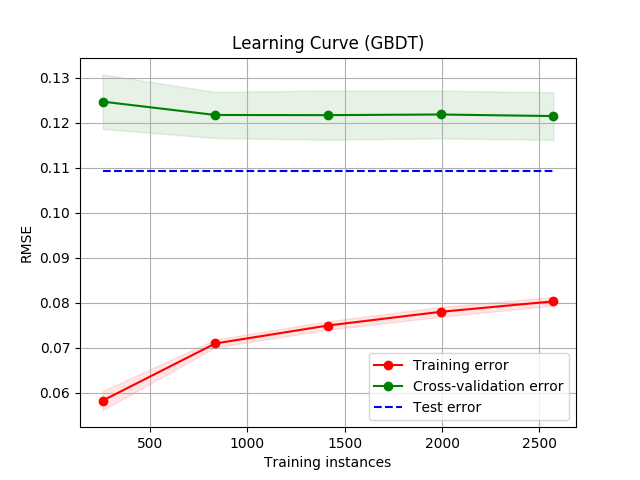
\includegraphics[width=0.8\linewidth]{img/query_learning_curve.png}
\caption{Learning curve of the query recency sensitivity model based on the number of training instances.}
\label{fig:query-curve1}
\end{figure}

\begin{figure}[h]
\centering
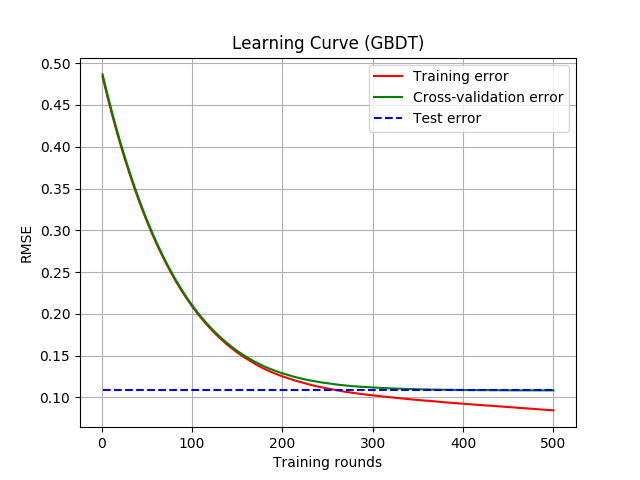
\includegraphics[width=0.8\linewidth]{img/query_learning_curve2.png}
\caption{Learning curve of the query recency sensitivity model based on the number of training rounds.}
\label{fig:query-curve2}
\end{figure}
